\chapter{Cosmic Rays and Neutrinos}
Cosmic rays alsmost exclusively refer to particles with a finite rest mass. The term \textit{rays} was historically wrongly attributed to these particles as they were thought to be mostly electromagnetic radiation.
The interest of cosmic rays within the field of particle physics and modern particle physics is clear: multiple new particles were discovered from the interactions at energies which were higher than most experiments could reach. Positrons, muons, pions and kaons were first discovered in cosmic ray experiments in the 1930s and 40s. Today, high-energy cosmic ray interactions are still of interest as the highest energies of these particles go beyond what is feasible at the most powerful accelorators such as the LHC. Neutrinos are expected be produced toghether with cosmic rays near the source or close to Earth making neutrino astronomy a powerful and important part of modern day astronomy. In this chapter I will give BLA BLA BLA. For a more exhaustive description of cosmic rays I refer the reader to \cite{Gaisser:2016uoy}.


\section{Discovery of cosmic rays}
With the use of electrometers, Victor Hess performed multiple ground-breaking balloon flight experiments in 1912 to prove that the amount of radiation increases with altitude \cite{hessnobel:1936}. This was in strong contradiction with the widespread belief that radiation on Earth's surface mostly originates from radioactive substances in its crust. Hess concluded that an extremely penetrating radiation existed. He described this radiation to be coming from space wich then enters Earth's atmosphere which proved to be correct but it was wrongfully attributed to electromagnetic radiation by Robert Millikan in the 1920s \cite{PhysRev.32.533}. 

Hess later ruled out the possibility that cosmic rays originate from the Sun as his observations showed no particular differences in night and day and during solar eclipses. In the late 1920s, first evidence was found that cosmic rays were charged due to a variation of their intensity with latitude \cite{clay:1927a}. This indicated that they were deflected by the geomagnetic field.

\section{What are cosmic rays?}
Cosmic rays are, almost exclusively, the collection of nuclei which are stripped of their electrons, making them electrically charged, heavy particles. Around 90\% of the particles are ionized hydrogen atoms, or protons. 9\% are alpha particles and 1\% are nuclei of heavier elements. There is a striking resemblance between the relative abundance of cosmic rays and elements in the Solar System as seen in Fig. \ref{fig:relabundance}. A much smaller fraction of incoming particles are electrons, positron and antiprotons.

\begin{figure}
\label{fig:relabundance}
\centering
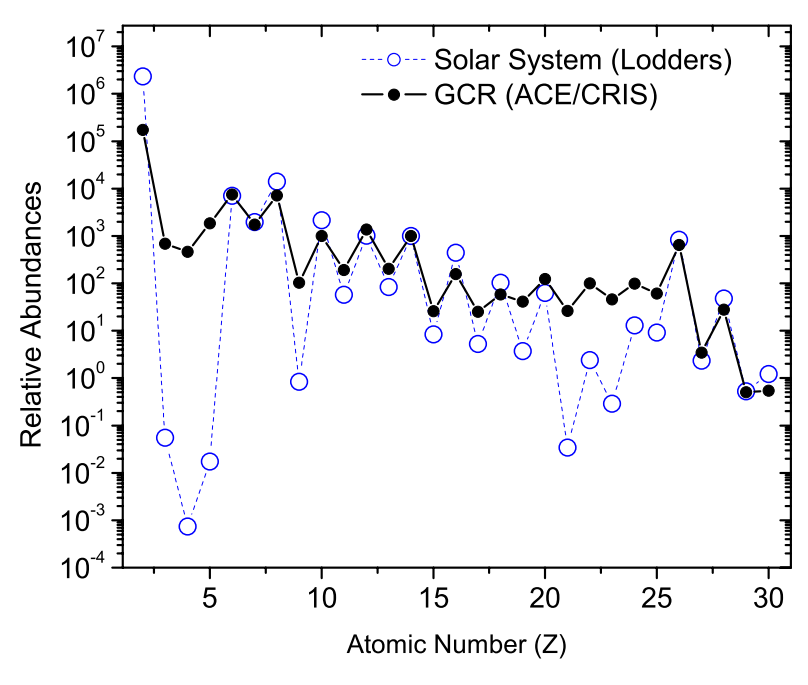
\includegraphics[width=0.7\textwidth]{./chapter3/img/relativeabundanceACE.png}
\caption{The cosmic ray elemental abundances measured on Earth compared to the solar system abundances, all relative to carbon = 100. Figure from ACE news archive \cite{ISRAEL2005201}.}
\end{figure}
There are however two important differences between cosmic rays and elements from our Solar System. Firstly, the two groups of elements Li, Be, B and Sc, Ti, V, Cr, Mn are many orders of magnitude more abundant in cosmic rays than in the solar system. This is due to their absence in stellar nucleosynthesis and are therefore not expected to be produced in large numbers. More massive cosmic rays (mainly C, O and Fe) can produce these nuclei in the process of \textit{spallation}. They are produced by collisions of cosmic rays with the interstellar medium. Therefore, these nuclei are sometimes referred to as \textit{secondary nuclei}.
The second difference is that nuclei with $Z>1$ are much more abundant with respect to hydrogen for cosmic rays. This phenomenon is not yet well understood but could be attributed to the difficulty to ionize hydrogen, necessary for acceleration processes.

The amount of cosmic rays seen on Earth is expressed in units of $\left[m^{-2} s^{-1} sr^{-1}\right]$. We can see in Fig. \ref{fig:spectrumCR} that the cosmic ray flux follows a energy power law spectrum:

\begin{equation}
dNdE \varpropto E^{-\gamma} dE,
\end{equation} 
where $\gamma$ is called the \textit{spectrum index}. Because of the steepness of the spectrum it is often multiplied by a higher power of energy\footnote{The broad range in both energy and flux should convince the reader that many types of detectors are necessary to study the behaviour of cosmic rays. Low-energy particles are abundant and high-energy particles are much more rare. Both the energy and the incoming flux will determine the type and size of the detector.}.

\begin{figure}
\label{fig:spectrumCR}
\centering
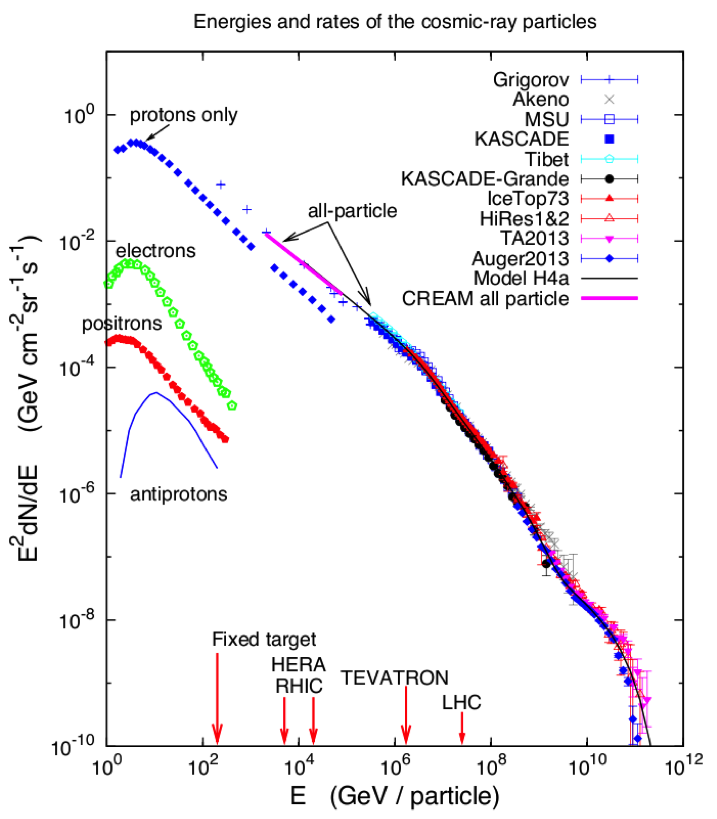
\includegraphics[width = 0.6\textwidth]{chapter3/img/spectrumCR.png}
\caption{Spectrum of cosmic rays at Earth. The all-particle spectrum measured by different experiments is plotted together with the proton-only spectrum. Subdominant contributions to the total flux from electrons, positrons and antiprotons as measured by the PAMELA experiment are also shown. Figure from \cite{Blasi:2013rva}.}
\end{figure}

We can divide the global spectrum in four regions. Between 10 GeV and 1 PeV the differential spectrum index is around -2.7. From 10 PeV to 1 EeV it is around -3.1. Above 10 EeV the spectrum again flattens to an index around -2.6 and an apparent cutoff region is present at around $10^{20}$ eV. The transition of this first to second region is referred to as the \textit{knee} at around 3 PeV. The second to third region transition is referred to as the \textit{ankle}. It is possible to describe the full cosmic-ray spectrum with sources within our galaxy. A more generally accepted theory is that the knee in the spectrum originates from the end of a population of particles which are accelerated within our Milky Way \cite{Gaisser:2013bla}. 

Second knee?

The origin of cosmic rays has been a topic of discussion for many years. We know now that most particles originate from sources in the local galaxy, having spent on average $10^7$ years in diffusive motion in the interstellar medium \cite{Gaisser:2013bla}. This is consistent with the resemblance of the relative abundances of cosmic rays and elements from our Solar System. However, there is no general consensus about the origin of the cosmic rays with energies above $3 \times 10^{18}$ eV. In the following, the abovementioned energy regions are discussed in more detail.

\subsection{Solar modulation}
In the Solar System a stream of charged particles is released from the Sun. This stream is mostly made up of electrons, protons and alpha particles with kinetic energies ranging between 0.5 and 10 keV. Within this solar wind plasma there is a magnetic field. Cosmic rays coming in to the Solar System interact with these particles and magnetic field. The influence is greatest on particles with the lowest charges. This effect is called \textit{solar modulation}. In effect, we see a strong suppression of cosmic rays at energies of 10 GeV and below.

\subsection{Galactic component}
The most probable acceleration mechanism for cosmic rays originating from our Galaxy is by shocks driven by expanding supernova remnants \cite{0034-4885-64-4-201}. From the ratio of primary to secondary nuclei it can be inferred that cosmic rays travel distances thousands of times greater than the thickness of the disk of the Galaxy. There is also an apparent decrease in the amount of matter that is traversed by cosmic rays with higher energies than with lower. Higher-energy cosmic rays seem to spend less time in the Galaxy than lower-energy ones and suggests that cosmic rays are accelerated before most propagation occurs \cite{Gaisser:2016uoy}.

The way the spectrum is fit is not set in stone. Here I will use the convention used by Gaisser, Stanev and Tilav described used in reference \cite{Gaisser:2013bla}. The spectrum is subdivided in three populations. The first population corresponds to the particles accelerated by supernova remnants, with the knee signaling the cutoff of this population. The second population is a higher-energy galactic component of unknown origin. The third generation will be described in more detail in \ref{subsec:ankle}. Assuming that the primary spectrum depends on the \textit{magnetic rigidity}\footnote{An assumption which is experimentally favored over other assumptions. Rigidity is an appropriate variable for interpreting changes in the spectrum due to propagation and acceleration in magnetic fields.},

\begin{equation}
R = \frac{pc}{Ze},
\end{equation}
where $Ze$ is the charge of a nucleus of total energy $E_{tot} = pc$ and relates to the gyroradius of a particle in a given magnetic field $B$ as

\begin{equation}
\label{eq:gyro}
r_L = \frac{R}{B}.
\end{equation}
If there is a characteristic regidity, $R_e$ above which a particular acceleration process reaches a limit, then the feature will show up in total energy first for protons, then for helium and so forth for heavier nuclei according to

\begin{equation}
E_{tot} = Ze \times R_e.
\end{equation}
This effect is visualised in Fig. \ref{fig:fitsgaisser} and indicates that as one population reaches its maximum the composition becomes heavier. The second knee, reported by KASCADE-Grande \cite{Apel:2011mi} and GAMMA \cite{Garyaka:2008gs} could be explained with an ``iron knee'' bump.

\begin{figure}
\label{fig:fitsgaisser}
\centering
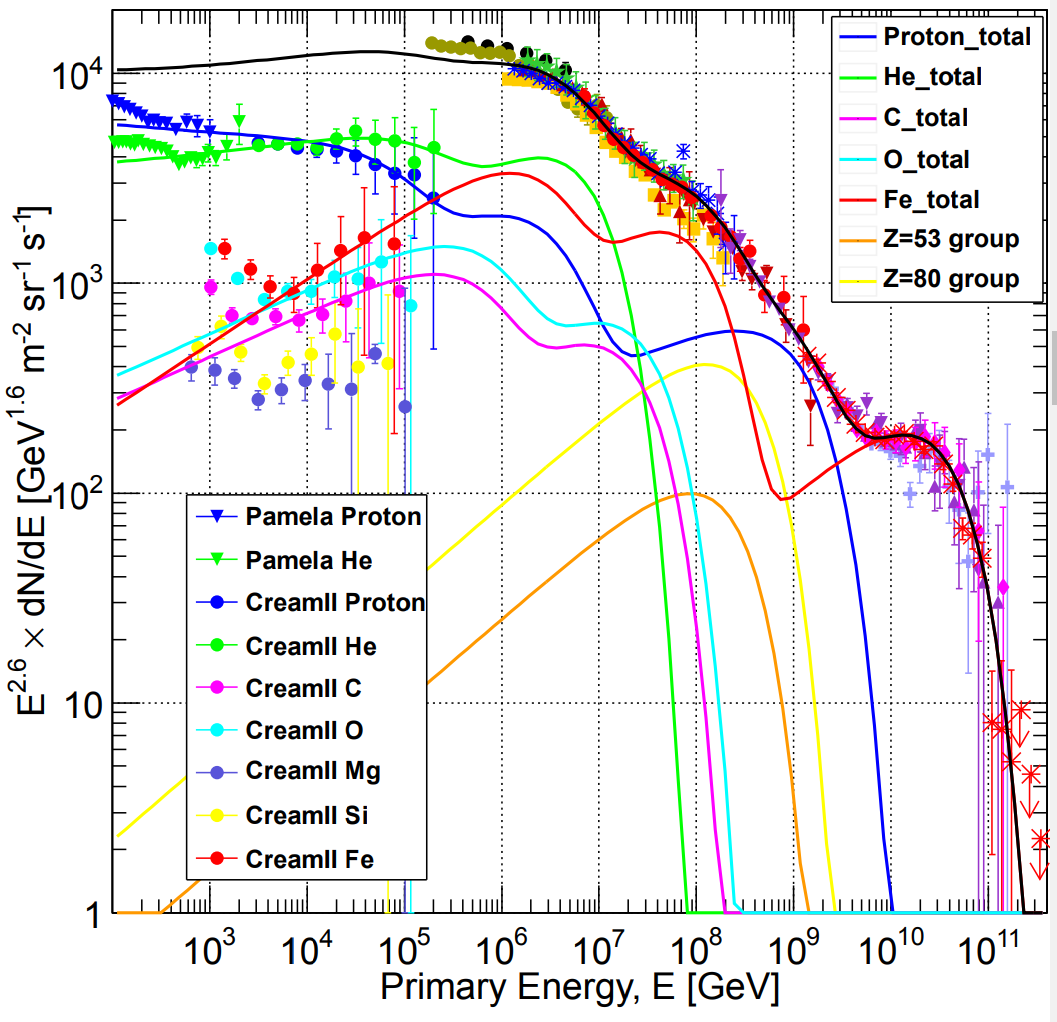
\includegraphics[width=0.48\textwidth]{chapter3/img/fit1gaisser.png}
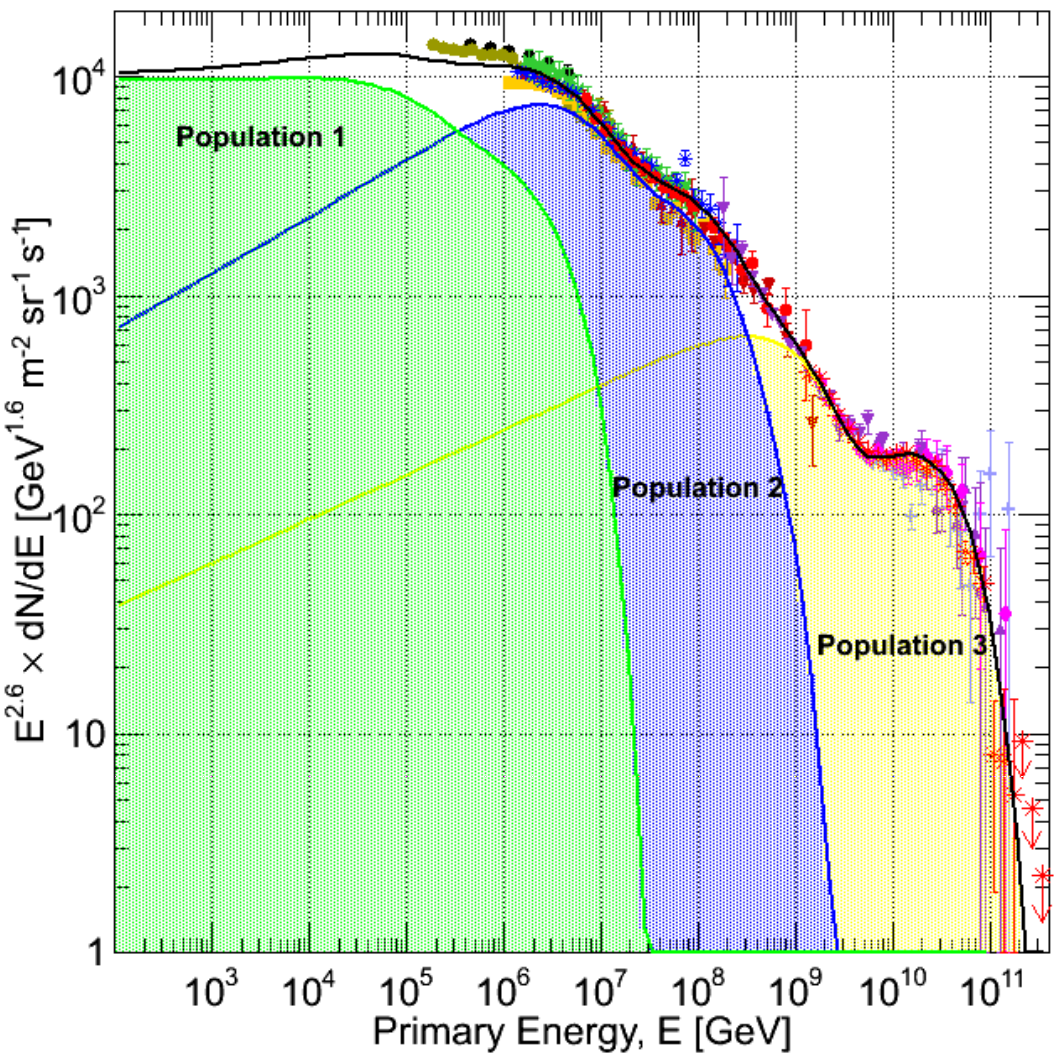
\includegraphics[width=0.48\textwidth]{chapter3/img/fit2gaisser.png}
\caption{Blub}
\end{figure}

%A schematic picture of our home galaxy, the Milky Way, is shown in Fig. 1.2. Most stars are concentrated in the galactic disc of height h $\approx$ 300 pc in the form of spiral arms. The disc is filled with warm atomic gas that consists to 90\% of H and to 10\% of He and has an average density n approx 1/cm3. It contains also an ordered magnetic field with strength B approx 3microG. The energy when the Larmor radius
\subsection{Extragalactic component}
The flux at the highest energies is exceedingly small. The number of events per year at energies above $5 \times 10^{19}$ eV is around one per square kilometer per century. There are only two experiments in the world capable of detecting the highest-energy cosmic rays in a statistical meaningful way: Telescope Array, located in the Northern Hemisphere (area of $\approx$700 km$^2$) and the Pierre Auger Observatory in the Southern Hemisphere (area of $\approx$3000 km$^2$).

Both experiments see a suppression of the flux above $6 \times 10^{19}$ eV. The exponential cutoff is consistent with the expected Greisen-Zatsepin-Kuzmin (GZK) effect \cite{Greisen:1966jv,Zatsepin:1966jv} where cosmic rays interact with the cosmic microwave background radiation (CMB)

\begin{equation}
\gamma_{CMB} + p \rightarrow \Delta^+ \rightarrow p + \pi^0
\end{equation} 
or

\begin{equation}
\gamma_{CMB} + p \rightarrow \Delta^+ \rightarrow n + \pi^+.
\end{equation}
Particles with energies above $5 \times 10^{19}$ eV would interact with the CMB, leading to an exponential cutoff (but if the incoming particles above these energies would be relatively young it is still possible for them to reach the detector). The Pierre Auger experiment reported to see higher compositions at the highest energies \cite{icrc2017:pa}. If the particle is a nucleus with A nucleons, then the GZK limit applies to its nucleons, which carry only a fraction 1/A of the total energy. For iron nuclei this would for example result in a limit of $2.8 \times 10^{21}$ eV. In contrast, the TA experiment interpreted their data as implying a light primary composition (mainly p and He) at the highest energies. Both experiments use a different interpretations for crucial quantities of these measurements and a thorough join analysis conducted by both experiments states that, at the current level of statistics and understanding of systematics, both data sets are compatible with being drawn from the same parent distribution \cite{PDG2018url}.

\begin{figure}
\label{fig:ankle}
\centering
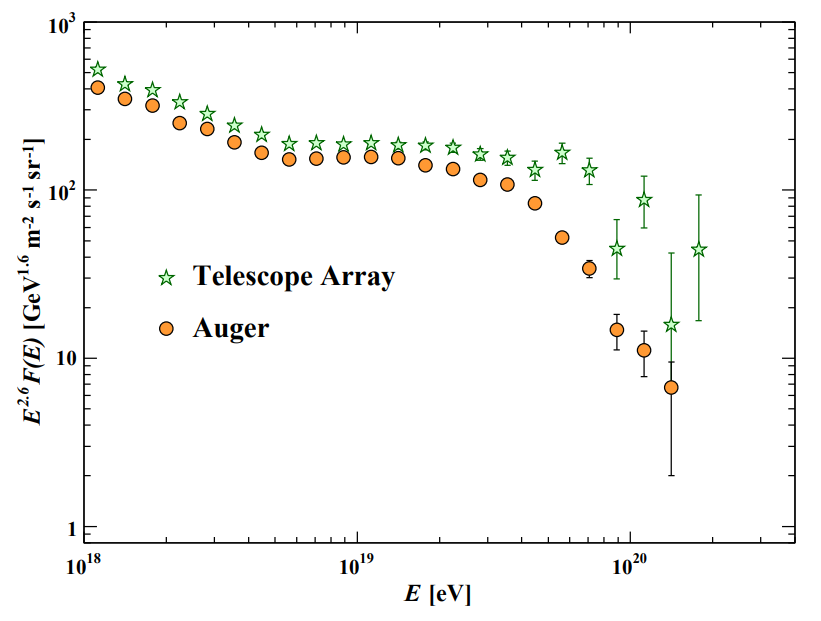
\includegraphics[width=0.6\textwidth]{chapter3/img/ankle.png}
\caption{Expanded view of the higest energy portion of the cosmic-ray spectrum from data of the Telescope Array and the Pierre Auger Observatory \cite{pdg2018}.}
\end{figure}
The Pierre Auger Observatory also reported evidence in an anisotripic distribution of the arrival directions of the highest-energy cosmic rays \cite{Aab:2017tyv} in a direction where the distribution of galaxies is relatively high and does not coincide with the galactic plane. These observations, together with our lack of known possible sources within our galaxy for these ultra-high energies shows compelling evidence that these particles have an origin from outside our galaxy. Dan misschien ook verwijzen naar paper van Waxman dat de hoogst energetische neutrinos en CRs linkt en zegt dat ze inconsistent zijn met galactische bronnen (2013)




"anti-matter but no anti-nuclei???"
Ook nog onduidelijkheden en waarom compositie zo moeilijk is. Compositie ook afhankelijk van energieschaal waar je naar kijkt bv.

Copy paste van Wikipedia:
 Data from the Fermi Space Telescope (2013)[3] have been interpreted as evidence that a significant fraction of primary cosmic rays originate from the supernova explosions of stars.[4] Active galactic nuclei also appear to produce cosmic rays, based on observations of a neutrino and gamma rays from blazar TXS 0506+056 in 2018.[5][6]



extragalactic neutrinos: IC paper


To put it simply, understanding cosmic rays and where they originate can help us answer fundamental questions about the origins of the universe, our galaxy and ourselves.
\section{Acceleration mechanism}
How cosmic rays got their signature slope in the energy spectrum and its intricate details have been under discussion for multiple decades. To this date there is no clear picture how these particles are accelerated in full detail. It is beyond the scope of this work to give a comprehensive overview of all possible acceleration mechanisms or possible sources. Most calculations are left out and for a more detailed discussion the reader is referred to specialized books or the references in the text.
\newline
The acceleration of the particles can be subdivided into two questions. First, where are the particles accelerated? Does it happen on large scales, cosmological distances in galaxies or near specific sources? Secondly, how are these particles exactly accelerated? What is the driving mechanism? Since primary cosmic rays are all electromagnetically charged particles these mechanisms should clearly be sought for in places where electric and/or magnetic fields play a dominant role.

\paragraph{Galactic accelerators}
With their approximate energy density around 0.5 eV/cm$^3$ in our local galaxy, the bulk of cosmic ray acceleration could very well be explained by \textbf{supernovae}. This density results into a total power of around

\begin{equation}
L_{CR} = 7 \times 10^{40} \textrm{ erg/s},
\end{equation}
where erg is a unit often used in astonomy\footnote{1 erg = $10^{-7}$ J.}. If one assumes a supernova explosion of around one per every 30 years then the total power output of type II supernovae with a mass output of around ten times the mass of the Sun at a velocity close to $5 \times 10^{8}$ cm/s would result in a power of

\begin{equation}
L_{SN} \backsim 3 \times 10^{42} \textrm{ erg/s}.
\end{equation}
These numbers are not set in stone and hold large uncertainties, but it shows that with an acceleration efficiency on the order of a couple of percent supernova explosions are a prominent source of energetic cosmic rays, if not the dominant one.

\paragraph{Extragalactic accelerators}
We will see in Section \ref{subsubsec:maxenergy} that the maximum energy from shock acceleration by a supernova remnant is insufficient to explain UHECR. As explained in Section \ref{subsubsec:fermiacceleration}, particles can be accelerated if the trajectory of the particles can be changed and energy can be transferred multiple times. The magnetic fields responsible for the course change of these particles has to be sufficient in magnitude in order for these particles not to escape and go beyond the grasp of the source responsible for the acceleration. This limitation is expressed by the gyroradius in the accelerator, $r_L = E/ZeB$ similar to Eq. \ref{eq:gyro}, requiring it to be smaller than the radius of the accelerator: $r_L < R$ or $E < ZeBR$.

Even if only qualitative, this relation provides an interesting criterion to idendify possible sources of UHECRs by looking at the accelerator related term $BR$. This was done in a classic paper by Hillas \cite{Hillas:1985is}, illustrated in the more recent Fig. \ref{fig:hillas}. Accelerators necessary to explain the amount of UHECRs are not populated (enough) in our galaxy, making them more likely to be of extra-galactic origin. \textbf{Active galactic nuclei, blazars and gamma ray bursts} (en andere als je die hebt toegevoegd later) are therefore also briefly explained.

\begin{figure}
\label{fig:hillas}
\centering
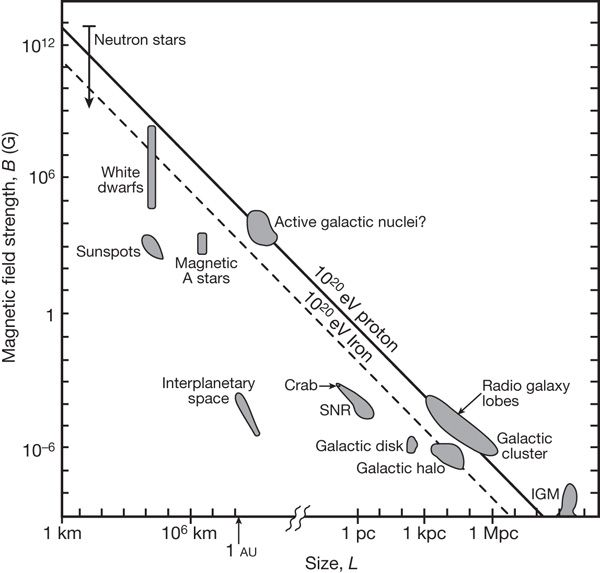
\includegraphics[width = 0.7\textwidth]{chapter3/img/Hillas.jpg}
\caption{The Hillas plot of potential cosmic ray accelerotors locates objects according to size and magnetic field. Objects to the left of the diagonal lines cannot accelerate particles to $10^{20}$ eV (proton: solid, iron: broken). Image obtained from \cite{Bauleo:2009zz}}
\end{figure}




\subsection{Supernova (remnants)}
Supernovae can be broadly subdivided into two categories: type I and type II. Type I supernova explosions happen in binary star systems. In those systems one of the two starts is a carbon-oxygen white dwarf which accretes matter from the second star. When the total mass of the white dwarf reaches the Chandrasekhar REF limit of around 1.44 solar masses it cannot longer hold itself under the gravitational pressure and collapses in on itself. Within seconds, the carbon component in the white dwarf starts nuclear fusion and enough energy is released to produce an explosion brighter than the Sun with a factor of around 5 billion. 
A resulting shock wave can reach up to around 3\% the speed of light.

Type II supernova explosions differ by being single star systems. When a star reaches the end of its lifecycle the subsequent fusion reactions reach to a halt. If the star has enough mass (at least 8 times the mass of the Sun), it is possible for the inner core to again reach the Chandrasekhar limit and collapse in on itself due to the lack of \textit{electron degeneracy}. Without the outward pressure of nuclear fusion reactions and the support of the core, the outer layers of the star collapse under the gravitational pressure. The compression of the electrons and protons into neutrons results into a very hot, dense, neutron core. The velocity of the inwards falling layers can reach to a staggering 23\% of the speed of light and recoil when hitting the remaining core. Neutrinos are produced in this violent core collapse and the outward going shockwave hits the remaining outer layers forming the supernova explosion \footnote{Astronomer Carl Sagan once said, "The nitrogen in our DNA, the calcium in our teeth, the iron in our blood, the carbon in our apple pies were made in the interiors of collapsing stars. We are made of starstuff."}.

Because of their brightness supernovae within our galaxy can be seen with the naked eye (provided they are not too far away). The last recorded supernova from our galaxy was by Johannes Kepler in 1604 but earliest recordings go back to 185 AD by Chinese astronomers\footnote{From observations of other galaxies supernovae are expected to occur, on average, once every thirty years. Not all of these will be visible to the naked eye, but would almost certainly be observable with modern astronomical telescopes.}.
\begin{figure}
\label{fig:supernova}
\centering
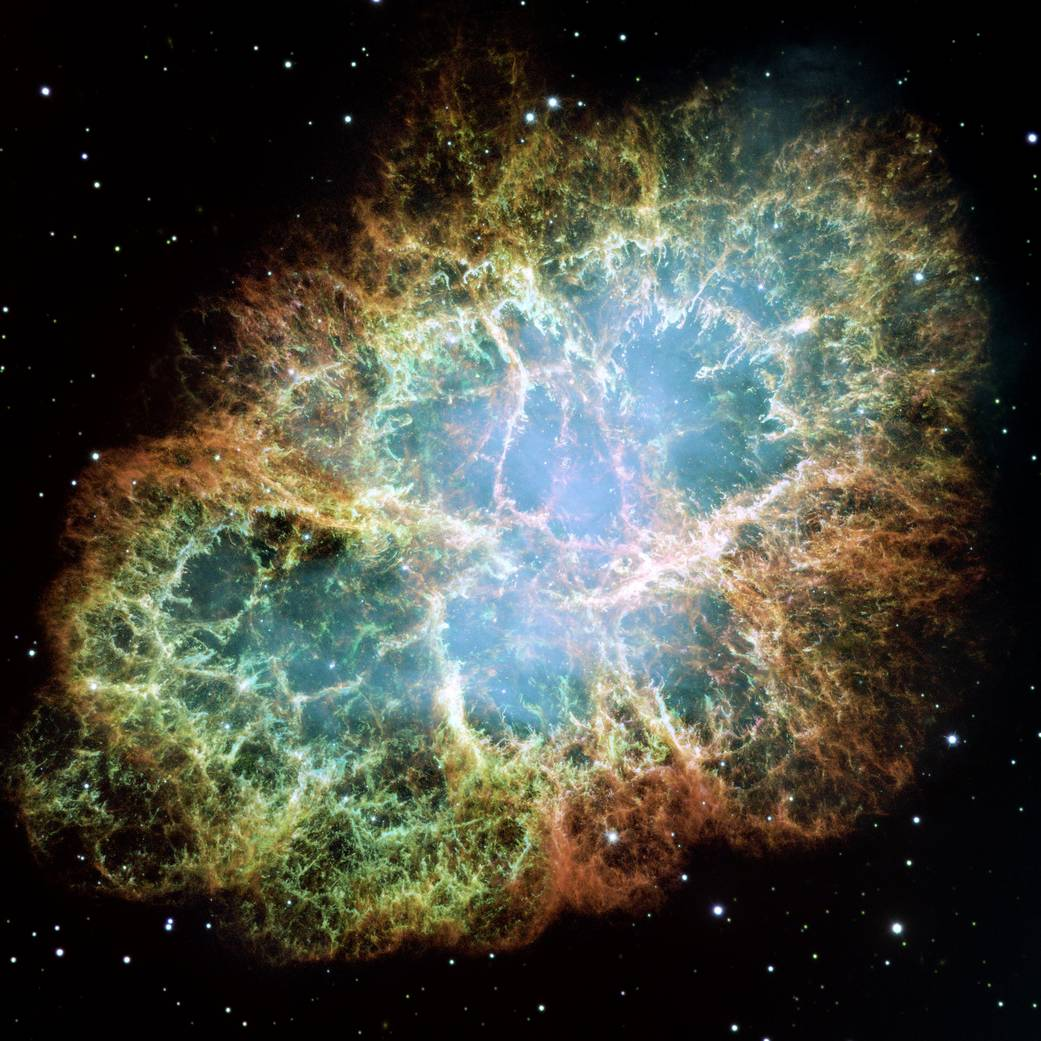
\includegraphics[width=0.48\textwidth,height=8cm]{chapter3/img/crabnebula.jpg}
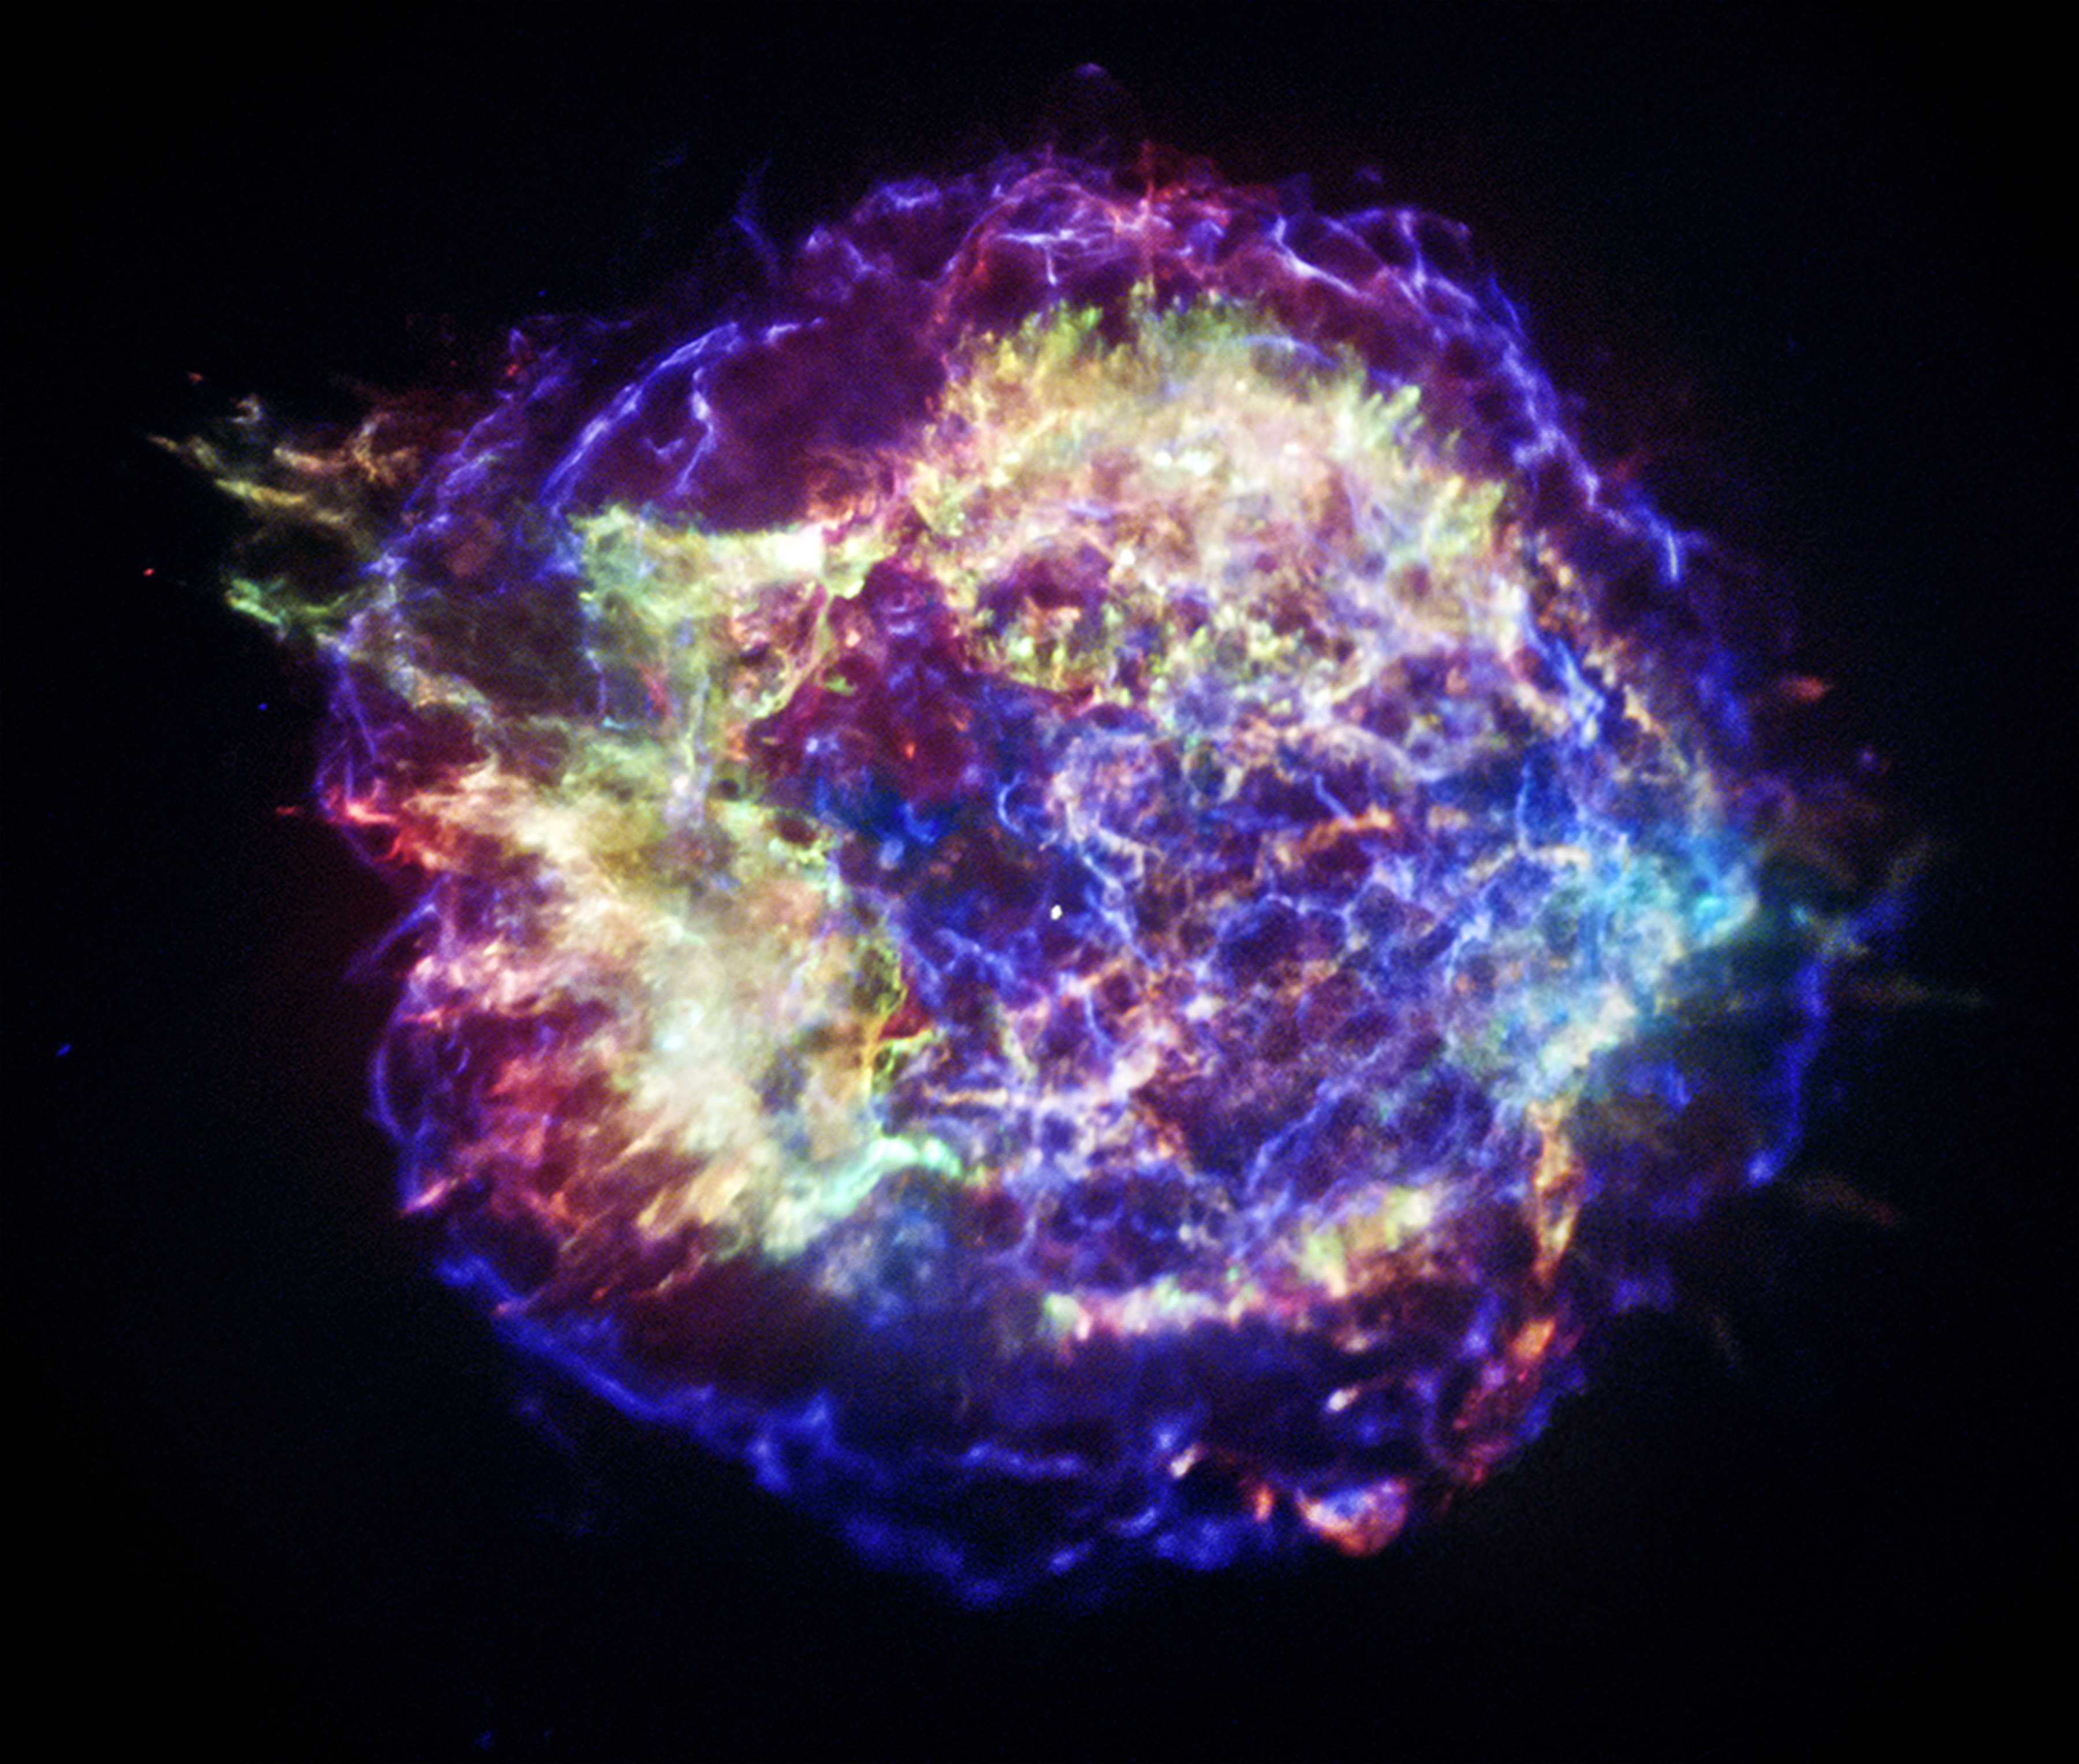
\includegraphics[width=0.48\textwidth,height=8cm]{chapter3/img/casa.jpg}
\caption{Left: the Crab Nebula is the supernova remnant approximately one thousand years old. The supernova was noted by Chinese astronomers in the year 1054 AD. Right: Chandra X-ray observatory picture of the Cassiopeia A supernova remnant (pictures from NASA).}
\end{figure}
\newline
The question remains how supernovae can serve as cosmic ray accelerators. In 1949, Enrico fermi proposed a mechanism where particles can gain energy by collisions with moving interstellar ionized gas clouds. Only later, it was realized that a large, plane shock front moving with a certain velocity is able to accelerated charged particles much more efficiently. This first mechanism results into an energy transfer proportional to the squared velocity of the cloud and is thus called \textit{second order Fermi acceleration}. Shock front acceleration energy transfer is proportional to the velocity and is called \textit{first order Fermi acceleration}. Supernova remnants provide an explanation for the origin of these shock fronts.


\subsubsection{First- and second-order Fermi acceleration}
\label{subsubsec:fermiacceleration}

Hoe van -2 naar -2.7???
Seems plausible all galactic CRs are accounted for my supernovae. This is supported with the realization that first-order Fermi acceleration naturally produces a spectrum of cosmic rays close to what is observed.

Suppose we have a magnetic cloud in the interstellar medium travelling with a certain velocity $\vec{V}$ and a particle with velocity $\vec{v}$ enters the cloud under an angle $\theta_1$ (see Fig. \ref{fig:cloud}). If we assume collisionless scattering can occur (no energy is dissipated from the particle to the cloud) due to the magnetic fields in the cloud, the magnitude of the momentum in the rest frame of the cloud will not change ($E'_1 = E'_2$, where we the apostrophe denotes the cloud rest frame). From special relativity we know that:

\begin{figure}
\label{fig:cloud}
\centering
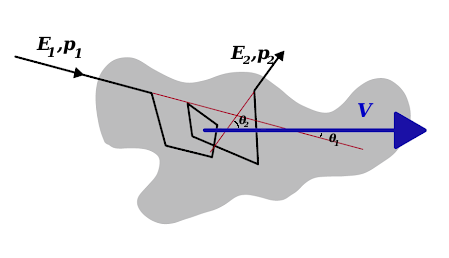
\includegraphics[width=0.48\textwidth]{chapter3/img/cloud.png}
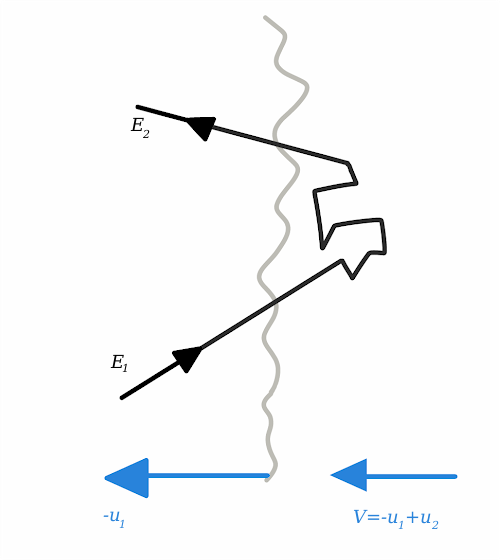
\includegraphics[width=0.48\textwidth]{chapter3/img/shock.png}
\caption{Left: magnetic cloud. Right: shock waves typically have magnetic inhomogeneities both preceding (downstream) and following them (upstream). If a charged particles travels trough the shock wave it can gain velocity through first-order Fermi acceleration. In the illustration a particle travels from upstream to downstream and back upstream. At every back and forth movement the particle effectively gains in energy. For a particle with a velocity $u_1$ relative to the shock front the front seems to come at him with velocity $-u_1$. The downstream medium has a velocity relative to the shock front of $u_2 < u_)1$ making it seem coming towards the particle with velocity $u_1-u2$.}
\end{figure}

\begin{equation}
\begin{split}
E'_1 &= \gamma \left(E_1 - p_{1,\parallel} V\right) \\
&= \gamma E_1 \left(1-\beta \cos \theta_1\right),
\end{split}
\end{equation}
with $\beta = V/c$ and $\gamma$ the Lorentz factor. Similarly and using $E'_1 = E'_2$

\begin{equation}
\begin{split}
E_2 &= \gamma E'_2 \left(1+\beta \cos \theta_2'\right)\\
&=\gamma^2 E_1 \left(1-\beta \cos \theta_1\right) \left( 1 + \beta \cos \theta_2'\right)
\end{split}
\end{equation}
and

\begin{equation}
\frac{\Delta E}{E} = \frac{E_2 -E_1}{E_1} = \frac{1 - 
\beta \cos \theta_1 + \beta \cos \theta_2' - \beta^2 \cos \theta_1 \cos \theta_2'}{1-\beta^2} -1.
\end{equation}
By hypothesis, the escaping particles are isotropic in the cloud frame: $\langle \cos \theta_2' \rangle = 0$. One can show that $\langle \cos \theta_1 \rangle = -\frac{\beta}{3}$ \cite{Gaisser:2016uoy}, leading to

\begin{equation}
\frac{\Delta E}{E} = \frac{4}{3} \frac{\beta^2}{1-\beta^2} \approx \frac{4}{3} \beta^2
\end{equation},
showing that for molecular clouds the energy gain is indeed proportional to the square of $\beta$ for second-order Fermi acceleration.
\newline
If a particle is incoming to an expanding shock (see Fig. \ref{fig:cloud}) $\langle \cos \theta_2'\rangle$ is equal to 2/3, leading to

\begin{equation}
\frac{\Delta E}{E} = \frac{\frac{4}{3}\beta + \frac{13}{9}\beta^2}{1-\beta^2} \approx \frac{4}{3} \beta,
\end{equation}
where $beta$ is now equal to $u_1 -u_2$ as explained in the caption of Fig. \ref{fig:cloud}. We have shown that for shock fronts the energy gain is indeed proportional to $\beta$ for first-order Fermi acceleration. From both the outcome as the discussion it is clear that the energy gain enters through relativistic effects, making the intuitive approach not straightforward.
\subsubsection{Power}
\subsubsection{Maximum energy}
\label{subsubsec:maxenergy}
\subsection{Active Galactic Nuclei}
\subsection{Blazars}
verwijzing naar txs!
\subsection{Gamma Ray Bursts}

\section{Neutrinos}
image with all kinds of neutrinos? Van Gary Binder
Ook iets zeggen over dat we ook extreem veel gamma ray studies hebben? Pg 236-237 in Gaisser.
Ook warom neutrinos zoveel handiger zijn dan fotonen en CRs
\section{Air shower}
\subsection{Cosmological}
\subsection{Solar}
\subsection{Atmospheric}
\subsubsection{Conventional}
\subsubsection{Prompt}
\subsection{Astrophysical}
Gaisser fig 2.10.
\section{Cosmic ray and neutrino detectors}
Heel kort: pg 5 Gaisser boek. Zo IC introduceren.

Ook dat plotje waarbij je toont dat neutrinos interessanter zijn in hoge E omdat fotonen onzichtbaar worden!

The IceCube Collaboration instead tested the principle using neutrinos. Neutrinos interact with matter through the weak force — one of the four fundamental forces of nature. The influence of the weak force is limited to minute distances. As a result, interactions between neutrinos and matter are extremely improbable, and a neutrino can easily traverse the entire Earth unimpeded. This poses a challenge for physicists trying to study these elusive particles, because almost every neutrino will simply pass through any detector completely unnoticed.




In neutral-current reactions neutrinos lose energy, but are not absorbed

hier tot pg 50?